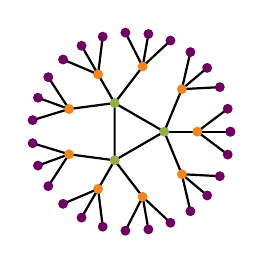
\begin{tikzpicture}[scale=0.42]
  \pgfmathsetmacro{\dtheta}{13.3333};

  % Draw the edges first

  \definecolor{level1}{RGB}{240,133,33}
  \pgfmathsetmacro{\dthetaParent}{3*\dtheta};
  \foreach \angle in {0, \dthetaParent, ..., 359}{ 
    \pgfmathsetmacro{\lbound}{\angle + \dtheta};
    \pgfmathsetmacro{\ubound}{\angle - \dtheta};

    \coordinate (node) at (\angle:2);

    \foreach \child in {\lbound, \angle, \ubound} {
      \draw[thick] (node) -- (\child:3);
    }

  }

  \definecolor{level2}{RGB}{148,174,74}
  \pgfmathsetmacro{\dthetaGrand}{3*\dthetaParent};
  \foreach \angle in {0, \dthetaGrand, ..., 359}{ 
    \pgfmathsetmacro{\lbound}{\angle + \dthetaParent};
    \pgfmathsetmacro{\ubound}{\angle - \dthetaParent};

    \coordinate (node) at (\angle:1);

    \foreach \parent in {\lbound, \angle, \ubound} {
      \draw[thick] (node) -- (\parent:2);
    }
  }

  \pgfmathsetmacro{\pang}{0};
  \pgfmathsetmacro{\qang}{\dthetaGrand};
  \pgfmathsetmacro{\rang}{2*\dthetaGrand};

  \draw[thick] (\pang:1) -- (\qang:1) -- (\rang:1) -- cycle;

  % Then draw the nodes

  \pgfmathsetmacro{\nodeRadius}{0.15};

  \definecolor{level0}{RGB}{110,0,95}
  \foreach \angle in {0, \dtheta, ..., 360}{
    \draw[draw=none, fill=level0] (\angle:3) circle (\nodeRadius);
  }

  \definecolor{level1}{RGB}{240,133,33}
  \pgfmathsetmacro{\dthetaParent}{3*\dtheta};
  \foreach \angle in {0, \dthetaParent, ..., 359}{ 
    \coordinate (node) at (\angle:2);
    \draw[draw=none, fill=level1] (node) circle (\nodeRadius);
  }

  \definecolor{level2}{RGB}{148,174,74}
  \pgfmathsetmacro{\dthetaGrand}{3*\dthetaParent};
  \foreach \angle in {0, \dthetaGrand, ..., 359}{ 
    \coordinate (node) at (\angle:1);
    \draw[draw=none, fill=level2] (node) circle (\nodeRadius);
  }
\end{tikzpicture}
